\section{Versuchsaufbau und Durchführung}

\begin{figure}[h]
\centering
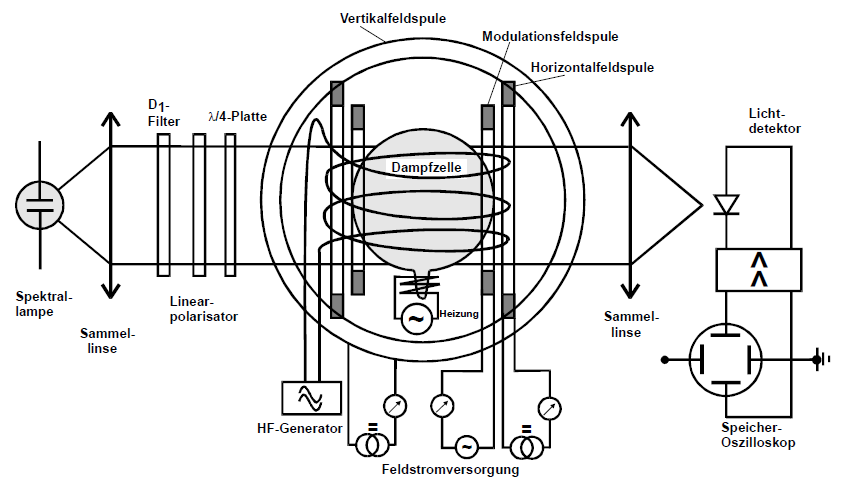
\includegraphics[width=\textwidth]{img/aufbau.png}
\caption{Schematischer Aufbau der Versuchsapparatur \cite{FP}.}
\label{aufbau}
\end{figure}

Der Versuch wird mit dem Aufbau, der in \autoref{aufbau} schematisch dargestellt ist, durchgeführt.
Dafür wird zunächst Rubidium erhitzt, sodass sich die Dampfzelle damit füllt. Das eingestrahlte
Licht einer Spektrallampe - eine Rb-Dampflampe in diesem Fall - passiert einen Interferenzfilter,
einen Polarisationsfilter und eine $\lambda/4$-Platte, um rechtszirkular-polarisiertes $D_1$-Licht
zu erhalten. Zur Messung der Transmission wird eine Photodiode als Lichtdetektor genutzt, das
Signal wird auf einem Oszilloskop dargestellt. Die Vertikalfeldspule dient dem Zwecke die
vertikale Komponente des Erdmagnetfeldes zu kompensieren.
Mit einer Sweep-Spule ("Modulationsfeldspule" in der Skizze) wird das Magnetfeld variiert, um die
Magnetfeldstärke bestimmen zu können, an denen induzierte Emission einsetzt und die Transmission
sinkt. An der Resonanzstelle besitzt die Transmission ein Minimum. Über einen Hf-Generator wird
die Modulationsfrequenz des Magnetfeldes eingestellt. Eine Horizontalfeldspule liefert außerdem
ein horizontales Magnetfeld, mit dem bei hohen Frequenzen die Feldstärke der Sweep-Spule auf die
Resonanzstellen verschoben werden kann. Daraus wird die Stärke des Erdmagnetfeldes, die
Lande-Faktoren und die Kernspins der Rubidiumisotope berechnet. Aus der Amplitude der Minima an
den Resonanzstellen wird das Isotopenverhältnis bestimmt. Durch Verändern der Amplitude des
Hochfrequenzfeldes bei festgehaltener Frequenz wird das Verhältnis der Relaxationsperioden
bestimmt. Ein angelegtes Magnetfeld wird so lange variiert bis der Einbruch in der Intensität
des eingestrahlten Lichts möglichst schmal wird. Dadurch wird der Effekt des Erdmagnetfeldes
kompensiert. Zu diesem Zweck ist der gesamte Versuch parallel zum Erdmagnetfeld auszurichten.
